% Options for packages loaded elsewhere
\PassOptionsToPackage{unicode}{hyperref}
\PassOptionsToPackage{hyphens}{url}
%
\documentclass[
]{article}
\usepackage{lmodern}
\usepackage{amssymb,amsmath}
\usepackage{ifxetex,ifluatex}
\ifnum 0\ifxetex 1\fi\ifluatex 1\fi=0 % if pdftex
  \usepackage[T1]{fontenc}
  \usepackage[utf8]{inputenc}
  \usepackage{textcomp} % provide euro and other symbols
\else % if luatex or xetex
  \usepackage{unicode-math}
  \defaultfontfeatures{Scale=MatchLowercase}
  \defaultfontfeatures[\rmfamily]{Ligatures=TeX,Scale=1}
\fi
% Use upquote if available, for straight quotes in verbatim environments
\IfFileExists{upquote.sty}{\usepackage{upquote}}{}
\IfFileExists{microtype.sty}{% use microtype if available
  \usepackage[]{microtype}
  \UseMicrotypeSet[protrusion]{basicmath} % disable protrusion for tt fonts
}{}
\makeatletter
\@ifundefined{KOMAClassName}{% if non-KOMA class
  \IfFileExists{parskip.sty}{%
    \usepackage{parskip}
  }{% else
    \setlength{\parindent}{0pt}
    \setlength{\parskip}{6pt plus 2pt minus 1pt}}
}{% if KOMA class
  \KOMAoptions{parskip=half}}
\makeatother
\usepackage{xcolor}
\IfFileExists{xurl.sty}{\usepackage{xurl}}{} % add URL line breaks if available
\IfFileExists{bookmark.sty}{\usepackage{bookmark}}{\usepackage{hyperref}}
\hypersetup{
  pdftitle={SPAN MRI Analytics Pilot Data Report: Lesion Volume Evaluation in Iowa Data},
  pdfauthor={Ryan P. Cabeen},
  hidelinks,
  pdfcreator={LaTeX via pandoc}}
\urlstyle{same} % disable monospaced font for URLs
\usepackage[margin=1in]{geometry}
\usepackage{color}
\usepackage{fancyvrb}
\newcommand{\VerbBar}{|}
\newcommand{\VERB}{\Verb[commandchars=\\\{\}]}
\DefineVerbatimEnvironment{Highlighting}{Verbatim}{commandchars=\\\{\}}
% Add ',fontsize=\small' for more characters per line
\usepackage{framed}
\definecolor{shadecolor}{RGB}{248,248,248}
\newenvironment{Shaded}{\begin{snugshade}}{\end{snugshade}}
\newcommand{\AlertTok}[1]{\textcolor[rgb]{0.94,0.16,0.16}{#1}}
\newcommand{\AnnotationTok}[1]{\textcolor[rgb]{0.56,0.35,0.01}{\textbf{\textit{#1}}}}
\newcommand{\AttributeTok}[1]{\textcolor[rgb]{0.77,0.63,0.00}{#1}}
\newcommand{\BaseNTok}[1]{\textcolor[rgb]{0.00,0.00,0.81}{#1}}
\newcommand{\BuiltInTok}[1]{#1}
\newcommand{\CharTok}[1]{\textcolor[rgb]{0.31,0.60,0.02}{#1}}
\newcommand{\CommentTok}[1]{\textcolor[rgb]{0.56,0.35,0.01}{\textit{#1}}}
\newcommand{\CommentVarTok}[1]{\textcolor[rgb]{0.56,0.35,0.01}{\textbf{\textit{#1}}}}
\newcommand{\ConstantTok}[1]{\textcolor[rgb]{0.00,0.00,0.00}{#1}}
\newcommand{\ControlFlowTok}[1]{\textcolor[rgb]{0.13,0.29,0.53}{\textbf{#1}}}
\newcommand{\DataTypeTok}[1]{\textcolor[rgb]{0.13,0.29,0.53}{#1}}
\newcommand{\DecValTok}[1]{\textcolor[rgb]{0.00,0.00,0.81}{#1}}
\newcommand{\DocumentationTok}[1]{\textcolor[rgb]{0.56,0.35,0.01}{\textbf{\textit{#1}}}}
\newcommand{\ErrorTok}[1]{\textcolor[rgb]{0.64,0.00,0.00}{\textbf{#1}}}
\newcommand{\ExtensionTok}[1]{#1}
\newcommand{\FloatTok}[1]{\textcolor[rgb]{0.00,0.00,0.81}{#1}}
\newcommand{\FunctionTok}[1]{\textcolor[rgb]{0.00,0.00,0.00}{#1}}
\newcommand{\ImportTok}[1]{#1}
\newcommand{\InformationTok}[1]{\textcolor[rgb]{0.56,0.35,0.01}{\textbf{\textit{#1}}}}
\newcommand{\KeywordTok}[1]{\textcolor[rgb]{0.13,0.29,0.53}{\textbf{#1}}}
\newcommand{\NormalTok}[1]{#1}
\newcommand{\OperatorTok}[1]{\textcolor[rgb]{0.81,0.36,0.00}{\textbf{#1}}}
\newcommand{\OtherTok}[1]{\textcolor[rgb]{0.56,0.35,0.01}{#1}}
\newcommand{\PreprocessorTok}[1]{\textcolor[rgb]{0.56,0.35,0.01}{\textit{#1}}}
\newcommand{\RegionMarkerTok}[1]{#1}
\newcommand{\SpecialCharTok}[1]{\textcolor[rgb]{0.00,0.00,0.00}{#1}}
\newcommand{\SpecialStringTok}[1]{\textcolor[rgb]{0.31,0.60,0.02}{#1}}
\newcommand{\StringTok}[1]{\textcolor[rgb]{0.31,0.60,0.02}{#1}}
\newcommand{\VariableTok}[1]{\textcolor[rgb]{0.00,0.00,0.00}{#1}}
\newcommand{\VerbatimStringTok}[1]{\textcolor[rgb]{0.31,0.60,0.02}{#1}}
\newcommand{\WarningTok}[1]{\textcolor[rgb]{0.56,0.35,0.01}{\textbf{\textit{#1}}}}
\usepackage{graphicx,grffile}
\makeatletter
\def\maxwidth{\ifdim\Gin@nat@width>\linewidth\linewidth\else\Gin@nat@width\fi}
\def\maxheight{\ifdim\Gin@nat@height>\textheight\textheight\else\Gin@nat@height\fi}
\makeatother
% Scale images if necessary, so that they will not overflow the page
% margins by default, and it is still possible to overwrite the defaults
% using explicit options in \includegraphics[width, height, ...]{}
\setkeys{Gin}{width=\maxwidth,height=\maxheight,keepaspectratio}
% Set default figure placement to htbp
\makeatletter
\def\fps@figure{htbp}
\makeatother
\setlength{\emergencystretch}{3em} % prevent overfull lines
\providecommand{\tightlist}{%
  \setlength{\itemsep}{0pt}\setlength{\parskip}{0pt}}
\setcounter{secnumdepth}{-\maxdimen} % remove section numbering
\usepackage{booktabs}
\usepackage{makecell}

\title{SPAN MRI Analytics Pilot Data Report: Lesion Volume Evaluation in Iowa
Data}
\author{Ryan P. Cabeen}
\date{2020-10-01}

\begin{document}
\maketitle

\hypertarget{full-table-of-lesion-volumes}{%
\section{Full Table of Lesion
Volumes}\label{full-table-of-lesion-volumes}}

\begin{Shaded}
\begin{Highlighting}[]
\KeywordTok{print}\NormalTok{(df[,}\KeywordTok{c}\NormalTok{(}\StringTok{"subject"}\NormalTok{, }\StringTok{"auto"}\NormalTok{, }\StringTok{"manual"}\NormalTok{, }\StringTok{"manual_personA"}\NormalTok{, }\StringTok{"manual_personB"}\NormalTok{)])}
\end{Highlighting}
\end{Shaded}

\begin{verbatim}
##    subject      auto manual manual_personA manual_personB
## 1   VH1919 20.979003 20.010           20.1          19.92
## 2   QC3809  9.865126 13.440           15.5          11.38
## 3   KX0579 28.525503 23.080           21.4          24.76
## 4   FR4979 15.568877 12.335           13.4          11.27
## 5   AM5399 19.787627 19.255           17.8          20.71
## 6   AM5398  0.000000  0.000            0.0           0.00
## 7   FR4960  0.000000  1.625            2.0           1.25
## 8   KX0560 15.045752 17.480           16.1          18.86
## 9   QC3810  1.667250  1.160            1.2           1.12
## 10  VH1900  2.409750  7.595            7.6           7.59
\end{verbatim}

\hypertarget{manual-volume-mean-and-standard-deviation}{%
\subsection{Manual Volume Mean and Standard
Deviation}\label{manual-volume-mean-and-standard-deviation}}

\begin{Shaded}
\begin{Highlighting}[]
\KeywordTok{mean}\NormalTok{(df}\OperatorTok{$}\NormalTok{manual)}
\end{Highlighting}
\end{Shaded}

\begin{verbatim}
## [1] 11.598
\end{verbatim}

\begin{Shaded}
\begin{Highlighting}[]
\KeywordTok{sd}\NormalTok{(df}\OperatorTok{$}\NormalTok{manual)}
\end{Highlighting}
\end{Shaded}

\begin{verbatim}
## [1] 8.555128
\end{verbatim}

\hypertarget{automated-volume-mean-and-standard-deviation}{%
\subsection{Automated Volume Mean and Standard
Deviation}\label{automated-volume-mean-and-standard-deviation}}

\begin{Shaded}
\begin{Highlighting}[]
\KeywordTok{mean}\NormalTok{(df}\OperatorTok{$}\NormalTok{auto)}
\end{Highlighting}
\end{Shaded}

\begin{verbatim}
## [1] 11.38489
\end{verbatim}

\begin{Shaded}
\begin{Highlighting}[]
\KeywordTok{sd}\NormalTok{(df}\OperatorTok{$}\NormalTok{auto)}
\end{Highlighting}
\end{Shaded}

\begin{verbatim}
## [1] 10.13184
\end{verbatim}

\newpage

\hypertarget{comparing-the-two-manual-segmentations}{%
\section{Comparing the two manual
segmentations}\label{comparing-the-two-manual-segmentations}}

\hypertarget{correlation}{%
\subsection{Correlation}\label{correlation}}

\begin{Shaded}
\begin{Highlighting}[]
\KeywordTok{cor}\NormalTok{(df}\OperatorTok{$}\NormalTok{manual_personA, df}\OperatorTok{$}\NormalTok{manual_personB)}
\end{Highlighting}
\end{Shaded}

\begin{verbatim}
## [1] 0.9693932
\end{verbatim}

\begin{Shaded}
\begin{Highlighting}[]
\KeywordTok{cor.test}\NormalTok{(df}\OperatorTok{$}\NormalTok{manual_personA, df}\OperatorTok{$}\NormalTok{manual_personB)}
\end{Highlighting}
\end{Shaded}

\begin{verbatim}
## 
##  Pearson's product-moment correlation
## 
## data:  df$manual_personA and df$manual_personB
## t = 11.168, df = 8, p-value = 3.7e-06
## alternative hypothesis: true correlation is not equal to 0
## 95 percent confidence interval:
##  0.8719917 0.9929606
## sample estimates:
##       cor 
## 0.9693932
\end{verbatim}

\hypertarget{root-mean-square-error}{%
\subsection{Root-mean-square error}\label{root-mean-square-error}}

\begin{Shaded}
\begin{Highlighting}[]
\KeywordTok{mean}\NormalTok{((df}\OperatorTok{$}\NormalTok{manual_personA }\OperatorTok{-}\StringTok{ }\NormalTok{df}\OperatorTok{$}\NormalTok{manual_personB)}\OperatorTok{**}\DecValTok{2}\NormalTok{)}\OperatorTok{**}\NormalTok{(}\FloatTok{0.5}\NormalTok{)}
\end{Highlighting}
\end{Shaded}

\begin{verbatim}
## [1] 2.22459
\end{verbatim}

\hypertarget{comparing-automated-and-manual-segmentations}{%
\section{Comparing automated and manual
segmentations}\label{comparing-automated-and-manual-segmentations}}

\hypertarget{correlation-1}{%
\subsection{Correlation}\label{correlation-1}}

\begin{Shaded}
\begin{Highlighting}[]
\KeywordTok{cor}\NormalTok{(df}\OperatorTok{$}\NormalTok{manual, df}\OperatorTok{$}\NormalTok{auto)}
\end{Highlighting}
\end{Shaded}

\begin{verbatim}
## [1] 0.9570602
\end{verbatim}

\begin{Shaded}
\begin{Highlighting}[]
\KeywordTok{cor.test}\NormalTok{(df}\OperatorTok{$}\NormalTok{manual, df}\OperatorTok{$}\NormalTok{auto)}
\end{Highlighting}
\end{Shaded}

\begin{verbatim}
## 
##  Pearson's product-moment correlation
## 
## data:  df$manual and df$auto
## t = 9.338, df = 8, p-value = 1.412e-05
## alternative hypothesis: true correlation is not equal to 0
## 95 percent confidence interval:
##  0.8239203 0.9900762
## sample estimates:
##       cor 
## 0.9570602
\end{verbatim}

\hypertarget{root-mean-square-error-1}{%
\subsection{Root-mean-square error}\label{root-mean-square-error-1}}

\begin{Shaded}
\begin{Highlighting}[]
\KeywordTok{mean}\NormalTok{((df}\OperatorTok{$}\NormalTok{manual }\OperatorTok{-}\StringTok{ }\NormalTok{df}\OperatorTok{$}\NormalTok{auto)}\OperatorTok{**}\DecValTok{2}\NormalTok{)}\OperatorTok{**}\NormalTok{(}\FloatTok{0.5}\NormalTok{)}
\end{Highlighting}
\end{Shaded}

\begin{verbatim}
## [1] 2.997068
\end{verbatim}

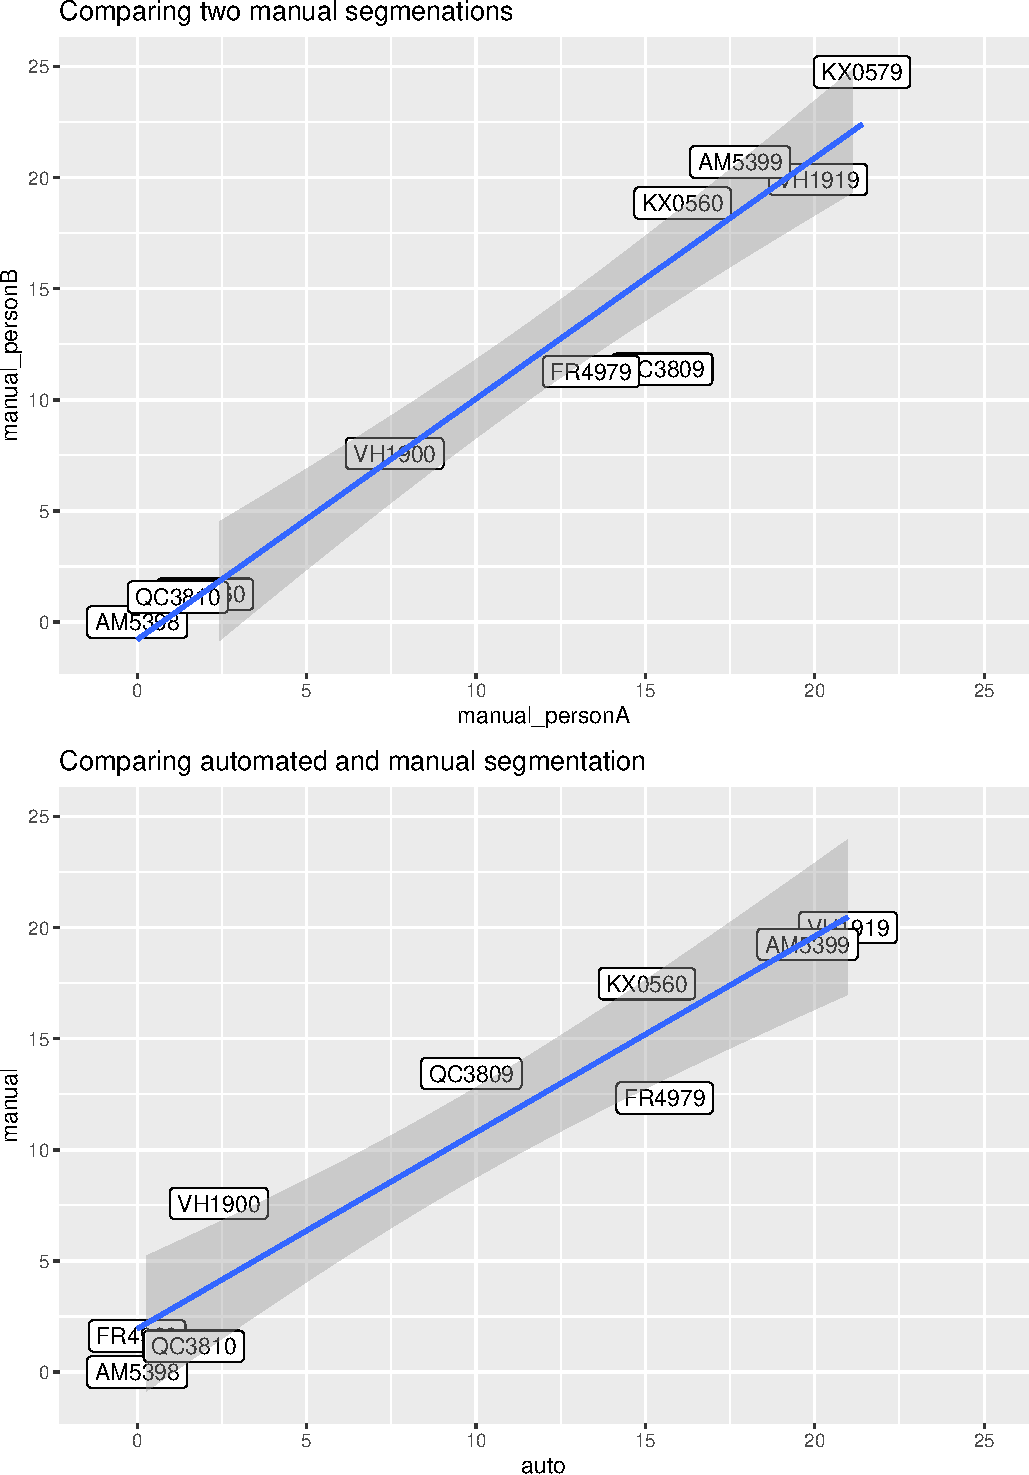
\includegraphics{paper_files/figure-latex/plot_all-1.pdf}

\end{document}
